\documentclass[tikz,border=2pt]{standalone}
\usepackage{amsmath}
\usepackage{pgfplots}
\pgfplotsset{compat=1.18}
\usetikzlibrary{arrows.meta}
\begin{document}
% Element-wise arithmetic pairs elements by position: x * y = (1*4, 2*5, 3*6) = (4, 10, 18);
% a single number is applied to every element: x - 1 = (0, 1, 2).
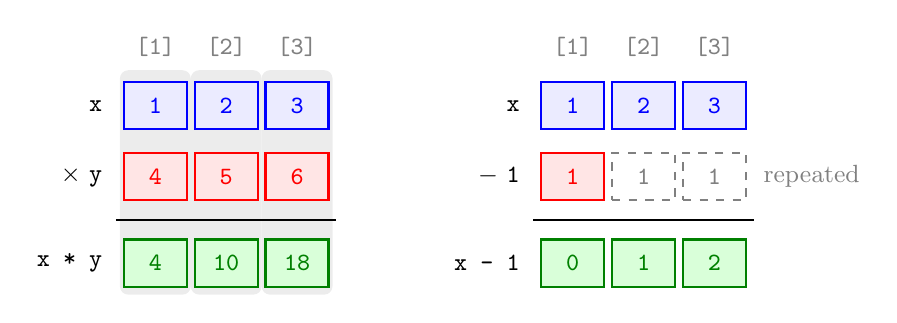
\begin{tikzpicture}[font=\small, >={Latex[length=2mm]},
  cell/.style={draw, thick, minimum width=8mm, minimum height=6mm, inner sep=0pt, font=\small\ttfamily}]
  % left panel: x * y
  \foreach \i in {1,2,3} {
    \fill[gray!15, rounded corners=3pt] (0.9*\i-0.45,-0.4) rectangle (0.9*\i+0.45,2.45);
    \node[gray, font=\small\ttfamily] at (0.9*\i,2.75) {[\i]};
  }
  \foreach \a/\b/\r [count=\i] in {1/4/4,2/5/10,3/6/18} {
    \node[cell, blue, fill=blue!8] at (0.9*\i,2) {\a};
    \node[cell, red, fill=red!10] at (0.9*\i,1.1) {\b};
    \node[cell, green!50!black, fill=green!15] at (0.9*\i,0) {\r};
  }
  \node[anchor=east] at (0.35,2) {\texttt{x}};
  \node[anchor=east] at (0.35,1.1) {$\times$\ \texttt{y}};
  \node[anchor=east] at (0.35,0) {\texttt{x * y}};
  \draw[thick] (0.4,0.55) -- (3.2,0.55);
  % right panel: x - 1
  \begin{scope}[xshift=5.3cm]
    \foreach \a/\r [count=\i] in {1/0,2/1,3/2} {
      \node[cell, blue, fill=blue!8] at (0.9*\i,2) {\a};
      \node[cell, green!50!black, fill=green!15] at (0.9*\i,0) {\r};
      \node[gray, font=\small\ttfamily] at (0.9*\i,2.75) {[\i]};
    }
    \node[cell, red, fill=red!10] at (0.9,1.1) {1};
    \node[cell, gray, dashed] at (1.8,1.1) {1};
    \node[cell, gray, dashed] at (2.7,1.1) {1};
    \node[anchor=east] at (0.35,2) {\texttt{x}};
    \node[anchor=east] at (0.35,0) {\texttt{x - 1}};
    \draw[thick] (0.4,0.55) -- (3.2,0.55);
    \node[anchor=east] at (0.35,1.1) {$-$\ \texttt{1}};
    \node[gray, anchor=west] at (3.2,1.1) {repeated};
  \end{scope}
\end{tikzpicture}
\end{document}
